\documentclass[10pt]{article}
\usepackage[a4paper,margin=1.6cm,top=1.3cm,bottom=1.3cm]{geometry}
\usepackage[T1]{fontenc}
\usepackage{lmodern}
\usepackage{microtype}
\usepackage{booktabs}
\usepackage{graphicx}
\usepackage{enumitem}
\usepackage{xcolor}
\usepackage[colorlinks=true,linkcolor=black,citecolor=black,urlcolor=blue]{hyperref}
\setlist{nosep,leftmargin=1.2em,topsep=1pt}
\setlength{\parindent}{0pt}
\setlength{\parskip}{3pt}
\pagestyle{empty}
\newcommand{\head}[1]{\par\smallskip{\large\bfseries #1}\par}
\newcommand{\sect}[1]{\par\smallskip{\bfseries\color{black!80} #1}\par}

\begin{document}
\head{Idea 9 PoC --- Bundled annual and Q1 reports}
\textit{Proof of concept, October 2026. Code: \texttt{idea09\_bundled\_reports/run.py} (argument: \texttt{sue\_xgb} or \texttt{sue\_rw}).}

\sect{Question and design}
Chinese firms must publish the annual report and the Q1 report by 30 April, and a growing share publish both on the
same day. When two earnings signals from the same firm arrive at once, do investors neglect one of them? This is a
within-firm test of limited attention (Hirshleifer and Teoh, 2003; Hirshleifer, Lim and Teoh, 2009), cleaner than
cross-firm clustering, which You and Zhang (2011) already study for China. The sample is 24{,}322 firm-years
(FY2005--2019) in three classes: \emph{same day} (4,977), \emph{same month, different day} (6,621) and \emph{separate
months} (12,724). The tests regress the release-month size-adjusted return on the annual (fiscal Q4) and Q1 XGBoost
surprises interacted with the class, controlling for the other surprise when it falls in the same month. Drift is
measured over months $+1$ to $+3$ after the later release. All regressions have month fixed effects, with SEs
clustered by month.

\begin{center}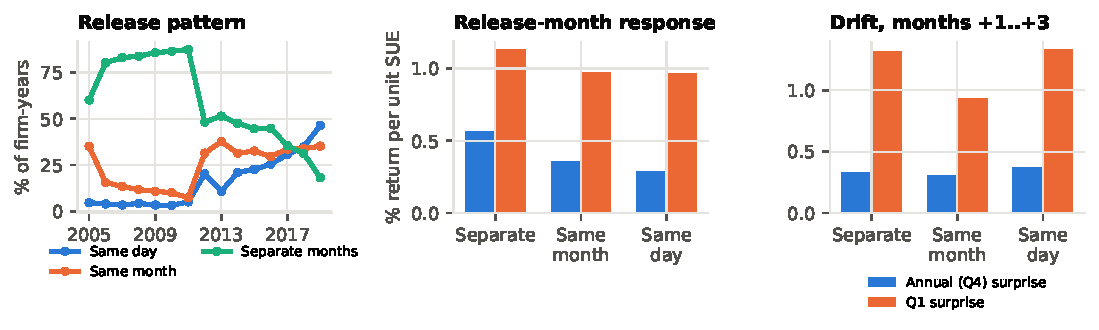
\includegraphics[width=0.97\textwidth]{results/fig_main_sue_xgb.pdf}\end{center}

\begin{center}\footnotesize
\setlength{\tabcolsep}{4pt}
\begin{tabular}{lccc|cc}
\toprule
 & \multicolumn{3}{c|}{Release-month response (\% per unit SUE)} & \multicolumn{2}{c}{Difference to separate ($t$)}\\
 & Separate & Same month & Same day & Same month & Same day\\
\midrule
Annual (Q4) surprise, XGBoost & 0.56 & 0.36 & 0.29 & $-0.21$ ($-1.7$) & $-0.28$ ($-3.1$)\\
Q1 surprise, XGBoost & 1.13 & 0.97 & 0.97 & $-0.16$ ($-0.6$) & $-0.16$ ($-0.7$)\\
Annual (Q4) surprise, SRW & 0.49 & 0.21 & 0.24 & $-0.28$ ($-2.5$) & $-0.25$ ($-3.4$)\\
\midrule
Drift of annual surprise, XGB / SRW & 0.33 / 0.10 & 0.30 / 0.22 & 0.37 / 0.36 & & $+0.04$ / $+0.26$ (0.1 / 1.1)\\
\bottomrule
\end{tabular}
\end{center}

\sect{Findings}
\begin{itemize}
\item \textbf{When both reports arrive together, the market roughly halves its response to the annual surprise.}
  The annual-report ERC falls from 0.56 to 0.29 for same-day bundles ($t=-3.1$), and the result holds with SRW
  surprises ($t=-3.4$). The response to the Q1 surprise is unchanged. Investors attend to the newer signal and
  discount the older one.
\item \textbf{The neglected part is not clearly recovered later.} The annual surprise drifts slightly more after
  bundles (SRW: 0.36 against 0.10), but not significantly. So the evidence fits either neglect or rational
  supersession, in which a fresh Q1 makes Q4 less relevant. Separating the two needs daily returns and longer
  windows.
\item \textbf{Bundling is strategic and habitual.} Firms with a negative annual surprise are 3.7--5.3 pp more likely
  to bundle (year FE, $t\geq5.6$). Bundlers earn lower subsequent returns ($-0.95\%$ over three months, $t=-2.1$).
  The choice is sticky: 59\% of last year's bundlers bundle again, against 13\% of others.
\item \textbf{A trend worth explaining.} Same-day bundling rose from about 4\% before 2011 to 49\% in FY2020. The jump
  in 2012 should be checked against exchange calendars to rule out a dating artifact in the panel.
\end{itemize}

\sect{Assessment and next steps}
This is the most promising Section~C idea: a new, cleanly defined attention test with a strong first result and a
built-in disclosure-strategy angle (``hiding'' bad annual news behind Q1). Next steps: (i) daily returns from Eikon
to measure announcement-window CARs and longer drift; (ii) validate the 2012 break with CNINFO filing timestamps;
(iii) use exchange-scheduled disclosure dates as an instrument for bundling, to address selection; (iv) test
whether analysts revise less on bundled annual surprises, which would link to Idea 1.
\end{document}
